\documentclass[../main.tex]{subfiles}

\begin{document}

\section{Introduction}
\label{sec: Introduction}

Forecasts of economic indicators such as GDP, inflation, and unemployment rate are important for policymakers, companies and investors.
However, accurate forecasts of these indicators are difficult since fluctuations in them are caused by complex interactions of various factors such as policies and economic activities.
The theory in the field of macroeconomics mainly deals with long-term fluctuations.  Therefore, the theory for short-term fluctuations has not been established yet.
Statistical time-series models have been used for short-term forecasts, but they are not sufficient.

The \emph{wisdom of the crowd}, which combines forecasts by many humans, is effective for short-term economic forecasts.
According to Ang, Bekaert and Wei~\cite{Ang2007}, the mean of expert forecasts collected by surveys is more accurate than macroeconomic models and time-series models.
Surowiecki~\cite{Surowiecki2004} has summarized many cases where the result of aggregating opinions of many people was accurate as the \emph{wisdom of the crowd}.

Economic forecasts by \emph{machine learning} have also attracted attention.
In recent years, the growth of computers and the Internet enabled us to handle large amounts of economic data.
By machine learning using these big data, it is possible to create complicated prediction models.
Several studies have reported that models based on \emph{artificial neural networks (ANN)} predicted inflation more accurately than the traditional time-series models~\cite{Choudhary2012, Moshiri2000, Nakamura2005}.

Both of a group of humans and machine make more accurate forecasts than the traditional methods.
However, the forecasting procedure is largely different in humans and machines.
While humans consider information such as economic conditions and policies when forecasting, machines make forecasts based on a statistical model constructed from past time series only.
For example, when an unprecedented financial crisis such as 2007--2008 occurred, machines can not forecasts the future well, while humans can forecast it flexibly.
In this manner, either one is not always more accurate.  Sometimes humans are more accurate, and in other times machines are.

This thesis aims to make more accurate forecasts by combining a group of humans and machine with harnessing their characteristics.
Combination methods for forecasts have been studied as \emph{ensemble methods} in the field of machine learning~\cite{Zhou2012} and as \emph{consensus forecasts} in the field of finance~\cite{Armstrong2001}.
In ensemble methods, although many of them include the training phase, combining methods of trained models can be applied to combinations with human forecasts.
Consensus forecasts aggregates forecast values by using simple average, weighted average and trimmed average.
In either method, however, there is no combining method that harnesses the good points of each forecaster.
It is impossible to emphasize human forecasts over the machine at financial crisis since traditional methods always use the same combination regardless of the situation (input).

\begin{figure}
  \centering
  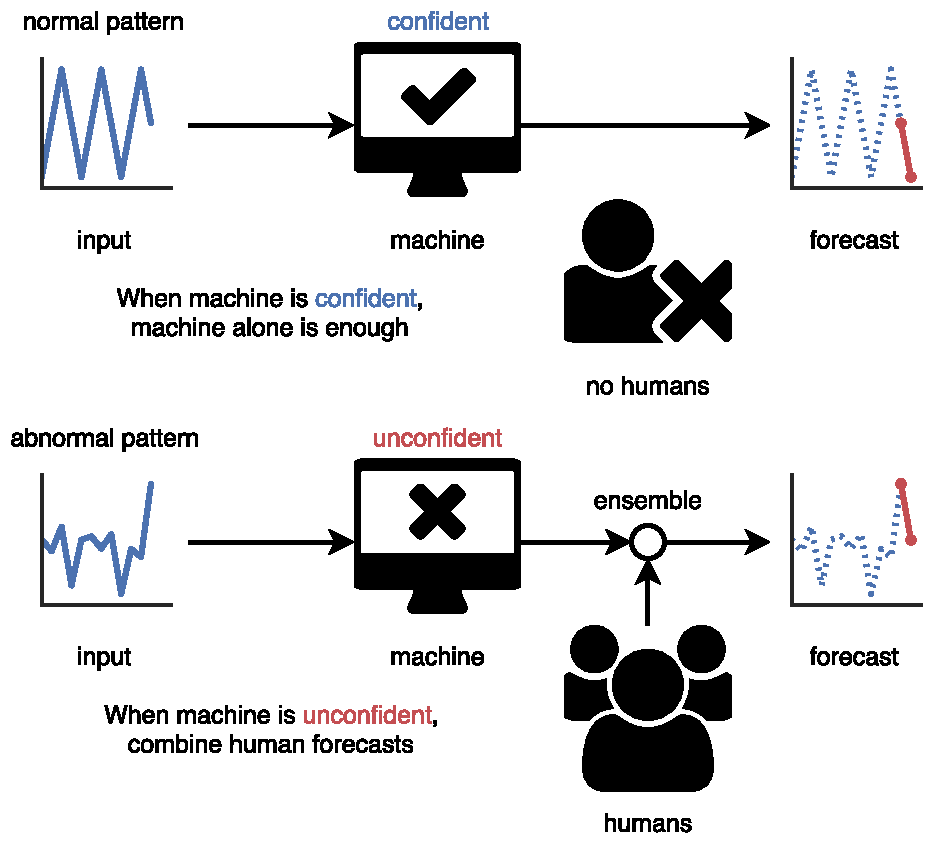
\includegraphics[width=\textwidth]{introduction-schematic}
  \caption{
    Schematic of a human-machine ensemble method
  }\label{fig: schematic}
\end{figure}

Therefore, this thesis proposes an ensemble method that emphasizes a machine if the machine is likely to forecast accurately and emphasizes humans otherwise.
Figure~\ref{fig: schematic} shows a schematic of a human-machine ensemble method this thesis proposes.
Machines are good at forecasting that follows patterns since they build a prediction model based on past data.
The upper part of the figure shows that when such a pattern is given, a machine forecast alone is enough since it can forecast the future well.
On the other hand, when a pattern not in the past is given, machines can not make a forecast well.
In such a case, the proposed method combines humans, who can forecast patterns not in the past, as shown in the lower part of the figure.
Through the above method, the proposed ensemble method take advantages of a machine and group of humans forecasts.
Specifically, we expand the existing model to express confidence in a forecast, which is represented by the expected error.
Based on the models, we propose an ensemble method that changes the combination of a machine and humans dynamically according to input.  It minimizes the expected errors of the forecasts by the ensemble.

We also conducted an experiment to apply the proposed method to actual inflation forecasts.
We made ANN prediction models using \emph{Long short-term memory (LSTM)} in the hidden layer as a machine.
And we used two survey data for economic forecasts as humans.
We also used traditional time-series models as benchmarks to compare them.
We prepared test set separately from the training set for evaluation.
We constructed seven ensembles and conducted verification of the proposed models, assessing forecast accuracy and confirmation of the behavior of the ensemble.

We obtained three empirical results as follows.
First, the proposed model, which express the expected error according to input, was valid on actual inflation forecasts.
Second, the proposed human-machine ensemble method made more accurate forecasts than each of a machine and group of humans in 4 out of 7.
Finally, the human-machine ensemble method emphasized human forecasts when a pattern not in the past was given as shown in Figure~\ref{fig: schematic}.

However, the human-machine ensemble method does not always behave as expected.
Therefore, we discuss the conditions to make use of the proposed ensemble method.
We also consider applications of the proposed method.

The rest of this thesis is organized as follows.
\ref{sec: Related Works} describes inflation forecasts, the wisdom of the crowd and ensemble methods as related works.
In \ref{sec: Human-Machine Ensemble Method}, we modeling forecasts of machines and humans, and propose a human-machine ensemble method.
\ref{sec: Experiment} describes the data set, forecasting models and evaluation methods used in the experiment.
\ref{sec: Empirical Results} contains the empirical results.
We discuss the scope and applications of the proposed method in \ref{sec: Discussion}.
Finally, \ref{sec: Conclusion} concludes.
\end{document}
